\documentclass[a4paper]{article}
\input{head}
\input{formulas.tex}
\begin{document}

%-------------------------------
%   TITLE SECTION
%-------------------------------

\fancyhead[C]{}
\hrule \medskip % Upper rule
\begin{minipage}{0.295\textwidth}
    \raggedright
    \footnotesize
    Maico Timmerman \hfill\\
    10542590\hfill\\
    maico.timmerman@gmail.com
\end{minipage}
\begin{minipage}{0.4\textwidth}
    \centering
    \large
    Homework Assignment 1\\
    \normalsize
    Natural Language Processing 1, 17/18\\
\end{minipage}
\begin{minipage}{0.295\textwidth}
    \raggedleft
    \today\hfill\\
\end{minipage}
\medskip\hrule
\bigskip

%-------------------------------
%   CONTENTS
%-------------------------------

\section*{Questions 1}
The  Chomsky Normal Form of the grammer is written as:

    \begin{table}[h]
        \centering
        \begin{tabular}{ccc}
            S &$\rightarrow$& NP VP\\
            S &$\rightarrow$& I X\\
            X &$\rightarrow$& NP VP\\
            NP &$\rightarrow$& Det N\\
            VP &$\rightarrow$& V NP\\
            PP &$\rightarrow$& Pre NP\\
            I &$\rightarrow$& \textit{I}\\
            VP &$\rightarrow$& \textit{ate}\\
            V &$\rightarrow$& \textit{ate}\\
            Det &$\rightarrow$& \textit{the} | \textit{a}\\
            N &$\rightarrow$& \textit{fork} | \textit{salad}\\
            Pre &$\rightarrow$& \textit{with}
        \end{tabular}
    \end{table}

\section*{Question 2}

\begin{enumerate}[label=(\alph*)]
    \item We can write the rules in cell \textbf{A}:

        \begin{table}[htpb]
            \centering
            \begin{tabular}{cccc}
                S &$\rightarrow$ & V Small & ($0.0096\approx 0.010$)\\
                S &$\rightarrow$ & V Obj Obj & ($0.0072\approx 0.007$)\\
                S &$\rightarrow$ & V Obj & (0.06)
            \end{tabular}
        \end{table}

        The rules in cell \textbf{B}:
        \begin{table}[htpb]
            \centering
            \begin{tabular}{ccll}
                S &$\rightarrow$ & Subj VP & (0.018)
            \end{tabular}
        \end{table}

        Resulting in a final tree:

        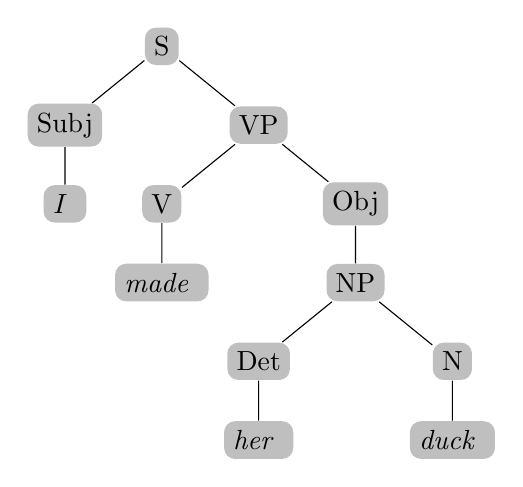
\begin{tikzpicture}[sibling distance=7em,
            level distance=1.0cm,
           every node/.style = {shape=rectangle, rounded corners,
             align=center, fill=black!25}]]
           \node {S}
             child { node {Subj}
               child { node {\textit{I} } } }
             child { node {VP}
               child { node {V}
                 child { node {\textit{made} } } }
               child { node {Obj}
                 child { node {NP}
                  child {node {Det} child { node {\textit{her} } } }
                  child {node {N} child { node { \textit{duck} } } } } } };
        \end{tikzpicture}

\end{enumerate}

\section*{Question 3}
\begin{enumerate}[label=(\alph*)]
    \item For every non-root we keep the highest incoming edge:

        \tikzstyle{edge} = [draw,thick]
        \tikzstyle{weight} = [font=\small]
        \tikzstyle{selected edge} = [draw,line width=5pt,-,red!50]
        \pgfdeclarelayer{background}
        \pgfsetlayers{background,main}
        \begin{tikzpicture}[shorten >=1pt,->, auto]
        \tikzstyle{vertex}=[circle,fill=black!25, minimum size=37pt,inner sep=0pt]

            \foreach \name/\x/\y in {root/1/5, likes/5/2, John/5/5, bagels/3/0, plain/0/0}
            \node[vertex] (\name) at (\x,\y) {\name};

            \foreach \from/\to/\label in {root/likes/15, likes/John/20, plain/likes/20, bagels/plain/15, likes/bagels/30}
                \path[edge] (\from) --  node [weight]{\label} (\to) ;

            \begin{pgfonlayer}{background}
                \foreach \source / \dest in {plain/likes, bagels/plain, likes/bagels}
                \path[selected edge] (\source.center) -- (\dest.center);
            \end{pgfonlayer}
        \end{tikzpicture}
        \vspace{2em}

    \item After completing the algorithm we result in:

        \begin{tikzpicture}[shorten >=1pt,->, auto]
        \tikzstyle{vertex}=[circle,fill=black!25, minimum size=37pt,inner sep=0pt]

            \foreach \name/\x/\y in {root/1/5, likes/5/2, John/5/5, bagels/3/0, plain/0/0}
            \node[vertex] (\name) at (\x,\y) {\name};

            \foreach \from/\to/\label in {root/likes/15, likes/John/20, bagels/plain/15, likes/bagels/30}
                \path[edge] (\from) --  node [weight]{\label} (\to) ;

        \end{tikzpicture}
\end{enumerate}

\section*{Question 4}
\begin{enumerate}[label=(\alph*)]
        \item
            We define a set $A$ as the set as created arcs, with initial value $A = \emptyset$. From this we start parsing according to Nivre's algorithm.

            \begin{table}[h]
                \centering
                \begin{tabular}{l|l|r|l}
                    Transition & Stack & Buffer & Arcs ($A$)\\
                    \hline
                    &  & A koala eats leafs and barks & $A (\emptyset)$\\
                    SHIFT &  A & koala eats leafs and barks & $A (\emptyset)$\\
                    LEFT-ARC(det) & & eats leafs and barks & $A = A \cup \text{det(koala, A)}$\\
                    SHIFT & koala & eats leafs and barks & $A$\\
                    LEFT-ARC(nsubj) & & leafs and barks & $A = A \cup \text{nsubj(eats, koala)}$\\
                    SHIFT & eats & leafs and barks & $A$\\
                    RIGHT-ARC(dobj) & eats leafs  & and barks & $A=A \cup \text{dobj(eats, leafs)}$\\
                    RIGHT-ARC(cc) & eats leafs and  & barks & $A =A \cup \text{cc(leafs, and)}$\\
                    REDUCE & eats leafs & barks & $A$\\
                    RIGHT-ARC(conj) & eats leafs barks & & $A=A\cup\text{conj(leafs, barks)}$\\
                    REDUCE & eats leafs & & $A$\\
                    REDUCE & eats & & $A$\\
                \end{tabular}
            \end{table}

            As our buffer is empty and there is only one word left on the stack, we see that the root of the sentence is ``eats'' and $A = \{\text{det(koala, A)}, \text{nsubj(eats, koala)}, \text{dobj(eats, leafs)}, \text{cc(leafs, and)}, \text{conj(leafs, barks)}, \text{root(root, eats)}\}$.
\end{enumerate}
\end{document}
% vim: ft=tex tw=0
